\documentclass[a4paper,14pt]{extarticle}
\usepackage{../../tex-shared/report-layout}

\renewcommand{\mylabnumber}{3}
\renewcommand{\mylabtitle}{Применение список и функций высших порядков для организации баз данных}
\renewcommand{\mysubject}{Методы и средства искусственного интеллекта}
\renewcommand{\mylecturer}{Сметанина Т.И.}

\begin{document}
\begin{titlepage}
    
    \thispagestyle{empty}
    
    \begin{center}
        
        Министерство науки и Высшего образования Российской Федерации \\
        Севастопольский государственный университет \\
        Кафедра ИС
        
        \vfill

        Отчет \\
        по лабораторной работе №\mylabnumber \\
        \enquote{\mylabtitle} \\
        по дисциплине \\
        \enquote{\MakeTextUppercase{\mysubject}}

    \end{center}

    \vspace{1cm}

    \noindent\hspace{7.5cm} Выполнил студент группы ИС/б-17-2-о \\
    \null\hspace{7.5cm} Горбенко К. Н. \\
    \null\hspace{7.5cm} Проверил \\
    \null\hspace{7.5cm} \mylecturer

    \vfill

    \begin{center}
        Севастополь \\
        \the\year{}
    \end{center}

\end{titlepage}

\section{Цель работы}
Исследование способов организации простых баз данных с помощью А-списков и
списков свойств, получение практических навыков использования и разработки
функций высшего порядка, изучение средств файлового ввода-вывода в языке Лисп.

\section{Постановка задачи}
Написать программу, обеспечивающую создание на диске базы данных. Структура базы
данных определяется одной из таблиц в соответствии с вариантом задания. В
функции программы должно входить:
\begin{itemize}
  \item создание базы данных;
  \item добавление записи в базу данных;
  \item сохранение базы данных на диске;
  \item загрузка базы данных в оперативную память;
  \item просмотр информации.
\end{itemize}

Вариант: корректировка данных в базе по начальному маршруту; вывод на экран информации о
маршруте, номер которого введен с клавиатуры; если таких маршрутов нет, выдать
на дисплей соответствующее сообщение.

\section{Ход работы}
Код программы:

\begin{lstlisting}
(defun main ()
  (defvar *db* nil)
  
  (insert "Севастополь" "Москва" "1")
  (insert "Евпатория" "Санкт-Петербург" "2")
  (insert "Москва" "Симферополь" "3")
  
  (print "БД после вставки:")
  (select*)
  
  (print "Сохранение в файл...")
  (savef "database.txt")
  (terpri)
  
  (print "Изменим номер маршрута по начальному пункту из Москвы и сохраним в файл:")
  (update (where :start "Москва") :number "99")
  (selectByNumber "99")
  (savef "database.txt")
  
  (terpri)
  (print "Попробуем найти несуществующий маршрут с номер 666:")
  (selectByNumber "666")
  
  (terpri)
  (print "Выгрузка из файла:")
  (loadf "database.txt")
  (select*)
)

(defun insert (start end number)
  (push (list :start start :end end :number number) *db*)
)

(defun savef (filename)
  (with-open-file (out filename :direction :output :if-exists :supersede)
    (with-standard-io-syntax
      (print *db* out)
    )
  )
)

(defun loadf (filename)
  (with-open-file (in filename)
    (with-standard-io-syntax
      (setf *db* (read in))
    )
  )
)

(defun select* ()
  (format t "~%~{~{~a:~a~%~}~%~}" *db*)
)

(defun where(&key start end number)
  #'(lambda (row)
       (and 
         (if start (equal (getf row :start) start) t)
         (if end (equal (getf row :end) end) t)
         (if number (equal (getf row :number) number) t)
       )
    )
)

(defun update (where-func &key start end number)
  (setf *db*
    (mapcar
     #'(lambda (row)
         (when (funcall where-func row)
           (if start (setf (getf row :start) start))
           (if end (setf (getf row :end) end))
           (if number (setf (getf row :number) number))
         )
        row
        )
      *db*
    )
  )
)

(defun selectByNumber (_number)
  (if (eq nil (setf rows (remove-if-not #'(lambda (row) (equal (getf row :number) _number)) *db*)))
    (print "Такого маршрута нет!")
    (print rows)
  )
)
\end{lstlisting}

Результат работы программы:
\begin{figure}[H]
    \centering
    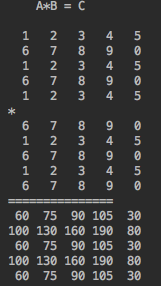
\includegraphics[width=.8\linewidth]{result}
    \caption{Результат работы программы}
    \label{fig:result}
\end{figure}

\section*{Выводы}
В ходе выполнения лабораторной работы были исследованы способы организации
простых баз данных с помощью А-списков и списков свойств, получены практические
навыки использования и разработки функций высшего порядка, изучены средства
файлового ввода-вывода в языке Лисп.

\end{document}